\chapter{Processor's Environment}
\label{ch:env}
The RISC processor is embedded in an environment (module RISCTop.v) connecting it with elements that are
FPGA-chip external, but whose are provided on the Spartan development board (Fig \ref{fig:cfg}). The
environment consists of an address decoder, a data multiplexer, and interfaces to the memory and
peripheral devices.
\begin{figure}[h!]
  \flushleft
  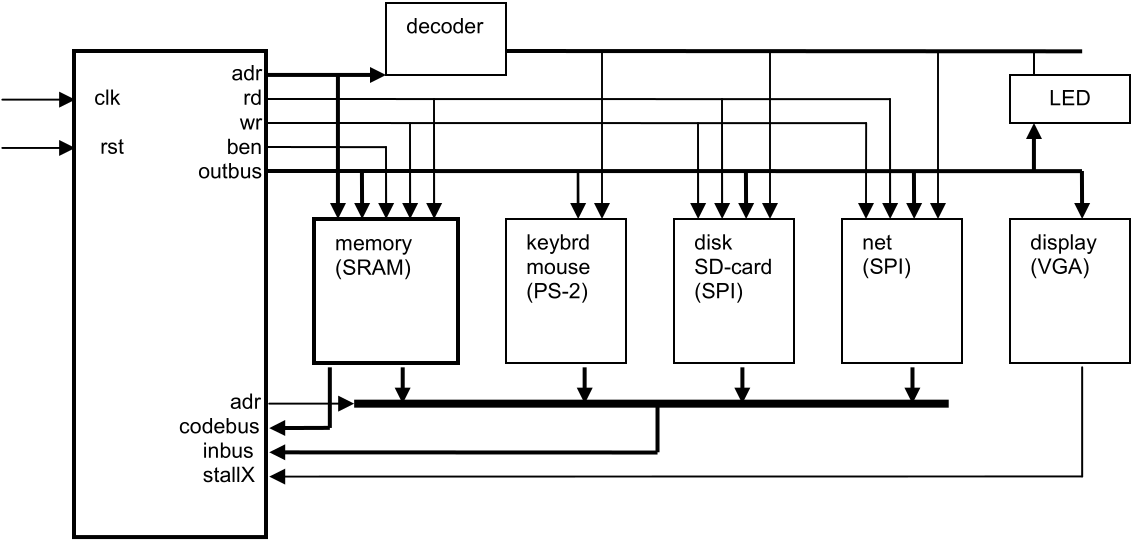
\includegraphics[width=1.1\textwidth]{i/G/0.png}
  \caption{The RISC configuration}
  \label{fig:cfg}
\end{figure}

The decoder for output and the multiplexer for input determine the various addresses of devices:
\begin{table}[h!]
  \centering
  \begin{tabular}{r l l l}
       & adr        & input                 & output \\\hline
     0 & 0FFFFFFC0H & millisecond counter   & reserved \\
     4 & 0FFFFFFC4H & switches              & LEDs \\
     8 & 0FFFFFFC8H & RS-232 data           & RS-232 data \\
    12 & 0FFFFFFCCH & RS-232 status         & RS-232 control \\
    16 & 0FFFFFFD0H & SPI data(SD-card,net) & SPI data(SD...) \\
    20 & 0FFFFFFD4H & SPI status            & SPI control \\
    24 & 0FFFFFFD8H & PS/2 keyboard \\
    28 & 0FFFFFFDCH & mouse
  \end{tabular}
\end{table}

The circuitry connecting with the SRAM is part of this module, whereas the drivers for the other
devices are described in separate modules. Note: The signals to and from devices must be listed in
the heading of the top module, which is not imported by any other module. Their pin numbers are
specified in a configuration file (.ucf). For details, the reader is referred to the program listing, as
several items are rather dependent on the given Spartan-3 board.

\section{The SRAM memory}
The design of the circuitry around a static RAM is quite straight forward. The only controls are a
read (SRoe) and a write enable signal (SRwe). Since the SRAM multiplexes data lines for input and
output, a tri-state driver (SRbuf) must be used on the FPGA. This is shown schematically in Fig \ref{fig:conn}.
\begin{figure}[h!]
  \centering
  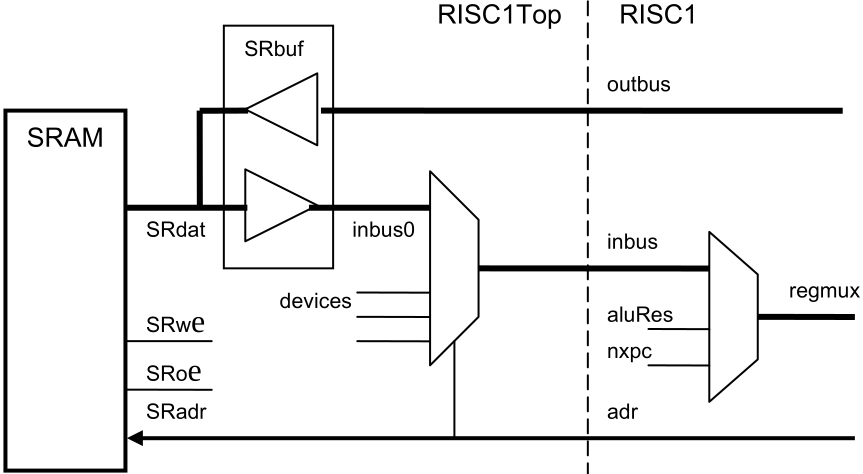
\includegraphics[width=\textwidth]{i/G/1.png}
  \caption{Connections between processor and SRAM}
  \label{fig:conn}
\end{figure}

However, there is a complication: the feature of byte-wise access. After all, the present RAM is 32
bits wide (actually there are two 512K x 16-bit chips in parallel). Evidently, some multiplexing is
unavoidable. The task is significantly eased by the chip's feature of four separate write enables,
one for each byte of a word. The selection of the byte affected is determined by address bits 0 an 1
(which are ignored in the case of word-access). This scheme is shown in Fig \ref{fig:sram}. The
codebus bypasses the multiplexers.
\begin{figure}[h!]
  \centering
  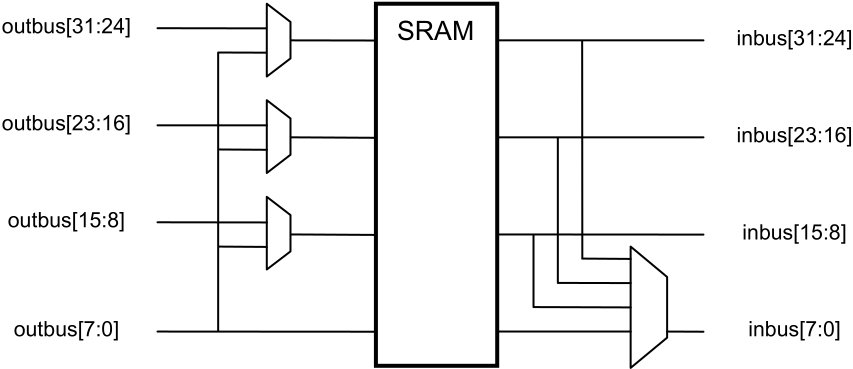
\includegraphics[width=.9\textwidth]{i/G/2.png}
  \caption{Multiplexers for SRAM byte access}
  \label{fig:sram}
\end{figure}

\section{Peripheral interfaces}
Each of the interfaces to external media is implemented as a separate module and can therefore
easily be exchanged. Modules are connected with the processor by the input and the output bus,
and by enable signals wr and rd.

\subsection{The PS/2 interface for the keyboard}
\label{sub:ps2}
PS/2 is mostly used for input devices. It uses 2 wires (apart from ground)., one for data, one for the
clock. It uses a synchronous transmission, and the clock is driven by the device. Here it is used for
the keyboard and the mouse (see Sect. 17.2.5). Transmission occurs in packets of 8 bits. An
optional third wire serves for output. It is not used in this application. The interface is very simple
and consists of an 8-bit buffer register. The following describes the interface for the keyboard.

A bit is shifted into the data register whenever the clock shows a falling edge, i.e. the clock signal
Q0 is low and the clock delayed by one cycle Q1 is high.
\begin{figure}[h!]
  \centering
  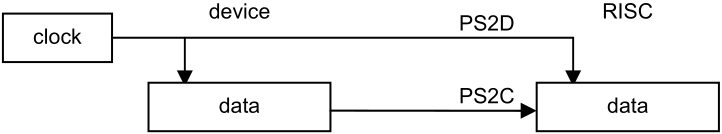
\includegraphics[width=.9\textwidth]{i/G/3.png}
  \caption{The PS/2 configuration}
  \label{fig:ps2}
\end{figure}

In the driver for the keyboard a 16-byte fifo buffer is inserted, forming a queue. This is necessary in order to
avoid loss of characters when the processor is tied up in computation.
\begin{verbatim}
module PS2(
 input clk, rst,
 input done, // "byte has been read"
 output rdy, // "byte is available"
 output shift, // shift in, transmitter
 output [7:0] data,
 input PS2C, // serial input
 input PS2D); // clock

reg Q0, Q1; // synchronizer and falling edge detector
reg [10:0] shreg;
reg [3:0] inptr, outptr;
reg [7:0] fifo [15:0]; // 16 byte buffer
wire endbit;

assign endbit = \~shreg[0]; //start bit reached correct pos
assign shift = Q1 \& \~Q0;
assign data = fifo[outptr];
assign rdy = \~(inptr == outptr);

always @ (posedge clk) begin
 Q0 <= PS2C; Q1 <= Q0;
 shreg <= (\~rst | endbit) ? 11'h7FF :
 shift ? {PS2D, shreg[10:1]} : shreg;
 outptr <= \~rst ? 0 : rdy \& done ? outptr+1 : outptr;
 inptr <= \~rst ? 0 : endbit ? inptr+1 : inptr;
 if (endbit) fifo[inptr] <= shreg[8:1];
end
endmodule
\end{verbatim}

\subsection{The Mouse}
Subsequently we present two Mouse interfaces. The first (MouseP) is based on the PS/2 Standard
and caters for most commercially available mice. The second (MouseX) is included here for
historical reasons. It was used by the computer Lilith in 1979, and used the same Mouse as its
ancestor Alto (at PARC, 1975). It is distinguished by a very simple hardware without its own
microprocessor, which is currently contained in most mice. This goes at a cost of a 9-wire cable.
But today, microprocessors are cheaper than cables. We include this interface here, because it
allows for a simple explanation of the principle of pointing devices.

The first interface uses the PS/2 Standard, that is, a 2-wire cable (not counting ground and power).
It complies with the commercial standard of pointing devices. Details are shown on module
MouseP.v.
\begin{verbatim}
module MouseP (input rst, clk,
 inout PS2C, PS2D,
 output [27:0] out);
endmodule
\end{verbatim}

The second interface described here is not based on any standard, but it features the same
interface to the software environment. Its principles are very simple and easily explained, and it
refrains from the use of a mouse-internal processor. The price for this simplicity is a cable with 7
wires (plus 2 for power and ground), namely 3 for 3 buttons, and 2 for each direction, x (left/right)
and y (up/down).

Let us first explain how signals indicating movements are derived. The key reason for the solution's
simplicity is that these signals are directly mirrored by the position of a cursor on the display. The
human user simply moves the Mouse until the cursor has reached the desired position (for
example, at a displayed object). Thereby, the human eye and hand are included in the feedback
loop providing the desired precision. This represents a very clever symbiosis between man and
computer.

An actual movement is recognized by a simple light sensor (we will restrict our observation to a
single coordinate x). The movement is transmitted to a wheel consisting of a transparent disc with
intransparent spokes. A light beam shines through the disk and is received by the light sensor.
Each time a spoke passes, the light is blocked. Any change in the sensor output signals a
movement (see Fig \ref{fig:wheel}). Unfortunately, this scheme does not allow to recognize the direction
of the movement (left or right). A second light and sensor solve this problem. The distance between
the two lights is half the distance of adjacent spokes.
\begin{figure}[h!]
  \centering
  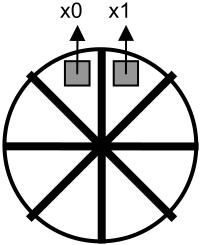
\includegraphics[width=.25\textwidth]{i/G/4.png}
  \caption{Wheel with spokes and sensors}
  \label{fig:wheel}
\end{figure}

The signal pair x0, x1 originating from a movement (with constant speed) to the left or to the right is
shown in Fig \ref{fig:sig}.
\begin{figure}[h!]
  \centering
  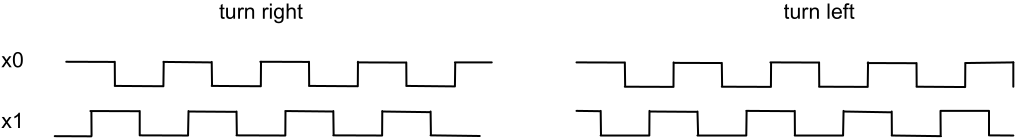
\includegraphics[width=\textwidth]{i/G/5.png}
  \caption{Signals resulting from movements}
  \label{fig:sig}
\end{figure}

The logic equations for movements to the left and right (or up and down) are derived from this signal
pair. For each signal a register records the state. Therefore it can be determined whether a move to
the left, or to the right, or no move had occurred. The sampling frequency is irrelevant, as long as it is
high enough. Let x01 be x00 delayed by one clock cycle, and x11 be x10 delayed by one cycle.
\begin{table}[h!]
  \centering
  \begin{tabular}{l  c c c c  c c c c  c c c c  c c c c}
    x00  & 0 & 0 & 0 & 0 & 0 & 0 & 0 & 0 & 1 & 1 & 1 & 1 & 1 & 1 & 1 & 1 \\
    x01  & 0 & 0 & 0 & 0 & 1 & 1 & 1 & 1 & 0 & 0 & 0 & 0 & 1 & 1 & 1 & 1 \\
    x10  & 0 & 0 & 1 & 1 & 0 & 0 & 1 & 1 & 0 & 0 & 1 & 1 & 0 & 0 & 1 & 1 \\
    x11  & 0 & 1 & 0 & 1 & 0 & 1 & 0 & 1 & 0 & 1 & 0 & 1 & 0 & 1 & 0 & 1 \\\hline
    right& 0 & 1 & 0 & 0 & 0 & 0 & 0 & 1 & 1 & 0 & 0 & 0 & 0 & 0 & 1 & 0 \\
    left & 0 & 0 & 1 & 0 & 1 & 0 & 0 & 0 & 0 & 0 & 0 & 1 & 0 & 1 & 0 & 0
  \end{tabular}
\end{table}

Every active right signal causes the 10-bit x counter to be incremented, and every left to be
decremented.

An identical circuit is used for the up/down direction, with its wheel set perpendicular to the first
wheel. Finally, the output is packed into a single word. 3 bits are taken by the keys, and 10 by each of
the two counters.
\begin{verbatim}
module MouseX(
 input clk,
 input [6:0] in,
 output [27:0] out);

 reg x00, x01, x10, x11, y00, y01, y10, y11;
 reg ML, MM, MR; // keys
 reg [9:0] x, y; // counters

 wire xup, xdn, yup, ydn;

 assign xup = \~x00\&\~x01\&\~x10\&x11 | \~x00\&x01\&x10\&x11 | x00\&\~x01\&\~x10\&\~x11 | x00\&x01\&x10\&\~x11;
 assign yup = \~y00\&\~y01\&\~y10\&y11 | \~y00\&y01\&y10\&y11 | y00\&\~y01\&\~y10\&\~y11 | y00\&y01\&y10\&\~y11;
 assign xdn = \~x00\&\~x01\&x10\&\~x11 | \~x00\&x01\&\~x10\&\~x11 | x00\&\~x01\&x10\&x11 | x00\&x01\&\~x10\&x11;
 assign ydn = \~y00\&\~y01\&y10\&\~y11 | \~y00\&y01\&\~y10\&\~y11 | y00\&\~y01\&y10\&y11 | y00\&y01\&\~y10\&y11;
 assign out = {1'b0, ML, MM, MR, 2'b0, y, 2'b0, x};

 always @ (posedge clk) begin
 x00 <= in[3]; x01 <= x00; x10 <= in[2]; x11 <= x10;
 y00 <= in[1]; y01 <= y00; y10 <= in[0]; y11 <= y10;
 MR <= \~in[4]; MM <= \~in[5]; ML <= \~in[6];
 x <= xup ? x+1 : xdn ? x-1 : x;
 y <= yup ? y+1 : ydn ? y-1 : y;
 end
endmodule
\end{verbatim}

\subsection{The SPI interface for the SD-card (disk) and the Net}
\label{sub:spi}
SPI (Standard Peripheral Interface) is similar to PS/2, and also synchronous. However, there may
be many participants. They are configured in a loop as shown in Fig \ref{fig:ring}, and the clock is
provided by a master, namely the RISC. SPI requires 3 wires (apart from ground).
\begin{figure}[h!]
  \centering
  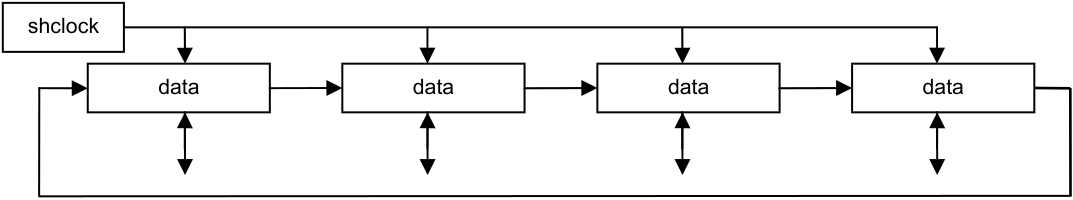
\includegraphics[width=.9\textwidth]{i/G/6.png}
  \caption{SPI-configuration as a ring}
  \label{fig:ring}
\end{figure}

Here, however, no use is made of SPI's ring topology. Instead, One master interface is serving both the disk
and the net. The connection is determined in module RISC5Top. The packet (and thus the shift register)
is 32 bits long

Transmission frequency is 0.4 MHz at startup (as required by the SD-card), and then is raised to
8.33 MHz. Details are shown in the respective program listing.
\begin{figure}[h!]
  \centering
  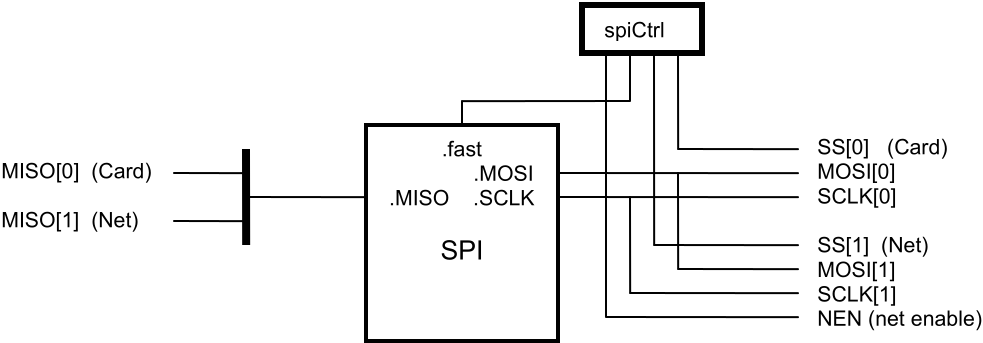
\includegraphics[width=\textwidth]{i/G/7.png}
  \caption{Connections between SPI, SD-card, and Net\\(see RISCTop5.v)}
  \label{fig:spi}
\end{figure}

// Motorola Serial Peripheral Interface (SPI) PDR 23.3.12 / 16.10.13
// transmitter / receiver of words (fast, clk/3) or bytes (slow, clk/64)
// e.g 8.33MHz or \~400KHz respectively at 25MHz (slow needed for SD-card init)
// note: bytes are always MSbit first; but if fast, words are LSByte first
\begin{verbatim}
module SPI(
 input clk, rst,
 input start, fast,
 input [31:0] dataTx,
 output [31:0] dataRx,
 output reg rdy,
 input MISO,
 output MOSI, SCLK);
endmodule
\end{verbatim}

The SPI specifications postulate that bytes are sent with the most significant bit first. This results in
a somewhat twisted scheme for shifting bits (see Fig \ref{fig:msb}).
\begin{figure}[h!]
  \centering
  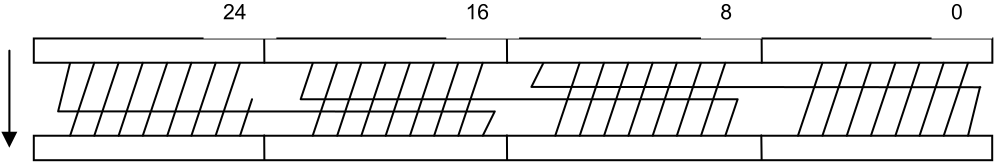
\includegraphics[width=\textwidth]{i/G/8.png}
  \caption{Shifting with MSB first}
  \label{fig:msb}
\end{figure}

\subsection{The display controller}
\label{sub:dispctrl}
A controller for a raster scan display feeds data from memory to the display. The data area in
memory is called frame buffer. It contains a fixed number of bits for each pixel on the screen. In this
case, there is exactly one bit per pixel, signalling black or white. For a 1024 x 768 pixel display
area, 96 Kbyte are required.

The pixel position on the display is not determined by an address. Instead, data are received by rhe
display purely sequentially, and the position is indirectly determined by two synchronization signals,
hsync (for horizontal sync) at the end of each line, and vsync (for vertical sync) at the end of every
frame. This scheme originates from cathode ray tube (CRT) monitors, where an electron beam is
sweeping the screen. It is deflected by magnetic fields, which require some time to sweep back.
The timing with retrace periods was retained for LCD displays as a legacy.

The heart of the controller consists of a data buffer (32 bits) fed from memory and shifted out bit by
bit to the display, and of two counters hcnt and vcnt, representing the horizontal and vertical
coordinates.The memory word address is derived from hcnt and vcnt:

vidadr = (hcnt DIV 32) + (vcnt * 32) + org

Every line consists of 1024 pixels (32 words). The challenge is to find a design with as few registers
and comparators as possible. There are two signals for suppressing video data: hblank, vblank.
They are needed for turning the light off durich retrace.
\begin{figure}[h!]
  \centering
  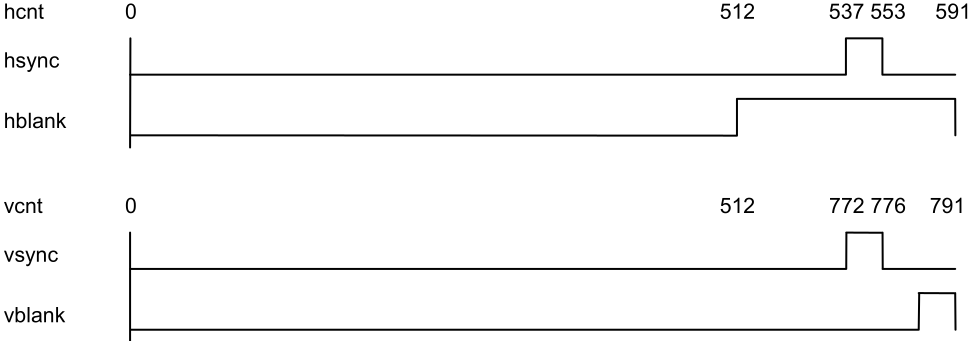
\includegraphics[width=.96\textwidth]{i/G/9.png}
  \caption{Synchronization and blanking signals}
  \label{fig:syn}
\end{figure}

Let us generalize this scheme to displays of w pixels per line and h lines per frame. Also, let w' be
the number of pixels per line including those of the retrace time, and h' be the number of lines
including the vertical retrace. Also, let the number of displayed frames per second be n. Then the
pixel frequency is

f = w' × h' × n.

This will in all probability be different from the system clock's frequency. Therefore the need arises
for a diffenernt pixel clock. It is generated by the FPGA's built-in digital clock manager (dcm). It
multiplies and divides the system clock by selectable factors. Note that the refresh rate may vary
within certain bounds for all brands of monitors. Therefore, a simple factor may be chosen for
division and multiplication. Examples:

(1024 x 768)
(1280 x 1024)

1182 x 791 x 60 = 56'097'720
1536 x 1280 x 60 = 117'964'800

rounded up to
rounded up to

60 MHz
125 MHz

The pixel buffer is fed from the video buffer driven by the system clock, and it is shifted and read by
the pixel clock. This makes a double-buffering necessary, as shown in Fig \ref{fig:vo}. Also the
counters are driven by this pixel clock. The numbers for hcnt and vcnt shown are, of course, device-
specific (see Fig \ref{fig:syn}).
\begin{figure}[h!]
  \centering
  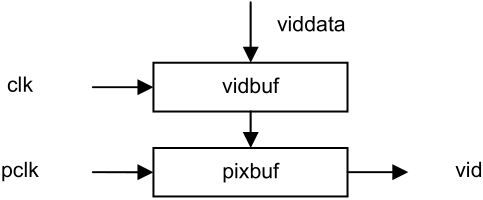
\includegraphics[width=.6\textwidth]{i/G/a.png}
  \caption{Buffering the video output}
  \label{fig:vo}
\end{figure}

\begin{verbatim}
module VID(
 input clk, clk25, inv,
 input [31:0] viddata,
 output reg req, // read request
 output hsync, vsync, // to display
 output [17:0] vidadr,
 output [2:0] RGB);
localparam Org = 18'b1101\_1111\_1111\_0000\_00; // DFF00
reg [9:0] hcnt, vcnt;
reg [4:0] hword; // from hcnt, but latched in the clk domain
reg [31:0] vidbuf, pixbuf;
reg hblank;
endmodule
\end{verbatim}

Both the display controller and the processor access memory directly. It therefore becomes
necessary to arbitrate in the case where both require access simultaneously, that is, to decide
which has priority. The decision is simple, because the display controller is time-critical and must
not be delayed. The processor, on the other hand, can easily be delayed by the already present
stalling scheme. The signal (wire) dspreq stalls the processor (stallX) and decides whether the
memory address (SRadr) should be taken from the processor (adr) or the display controller
(vidadr). The following multiplexer is placed in module RISCTop:

\begin{verbatim}
assign SRadr = dspreq ? vidadr : adr[19:2];
\end{verbatim}

\subsection{The RS-232 interface}
\label{sub:rs232}
RS-232 is an old standard for serial data transmission (see also Sect. 9.4). We chose to describe it
here in detail because of its frequent use and inherent simplicity. RS-232 uses 2 wires (apart from
ground), one for input (RxD) and one for output (TxD) as shown in Fig \ref{fig:rs232cfg}. Data are
transmitted in packets of a fixed length, here of length 8, i.e. byte-wise.
\begin{figure}[h!]
  \centering
  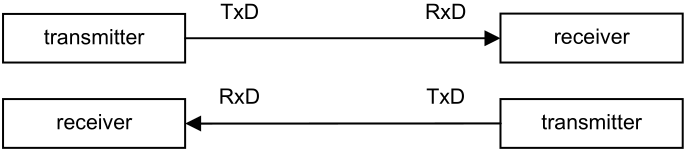
\includegraphics[width=.9\textwidth]{i/G/b.png}
  \caption{RS-232 configuration}
  \label{fig:rs232cfg}
\end{figure}
Since there is no clock wire,
bytes are transmitted asynchronously. Their beginning is marked by a start-bit, and at the end a
stop-bit is appended. Hence, a packet is 10 bits long (see Fig \ref{fig:rs232pac}). Within a packet,
transmission is synchronous, i.e. with a fixed clock rate, on which transmitter and receiver agree.
The packet length is short enough to admit slight deviations. The standard defines several packet
lengths and many clock rates. Here we use a rate of 19200 or 115200 bit/s.
\begin{figure}[h!]
  \centering
  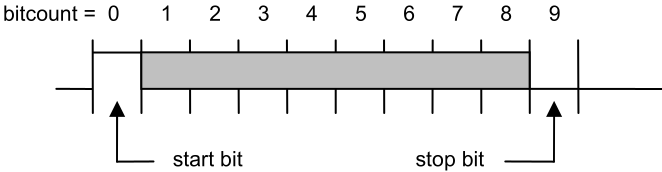
\includegraphics[width=.96\textwidth]{i/G/c.png}
  \caption{RS-232 packet format}
  \label{fig:rs232pac}
\end{figure}

The input signal start triggers the state machine by setting register run. The transmitter has 2
counters and a shift register. Counter tick runs from 0 to 1302, yielding a frequency of 25’000 / 1302
= 19.2 KHz, the transmission rate for bits. The signal endtick advances counter bitcnt, running from
0 to 9 (the number of bits in a packet). Signal endbit resets run and the counter to 0. Signal rdy
indicates whether or not a next byte can be loaded and sent.

\begin{verbatim}
module RS232T(
 input clk, rst, // system clock, 25 MHz
 input start, // request to accept and send a byte
 input [7:0] data,
\end{verbatim}

The receiver is structured very similarly with 2 counters and a shift register. The state machine is
triggered by an incoming start bit at RxD. The state rdy is set when the last data bit has been
received, and it is reset by the done signal, generated when reading a byte. The line RxD is
sampled in the middle of the bit period rather than at the end, namely when midtick = endtick/2.
\begin{verbatim}
 output rdy, // status
 output TxD); // serial data

wire endtick, endbit;
reg run;
reg [11:0] tick;
reg [3:0] bitcnt;
reg [8:0] shreg;

assign endtick = tick == 1302;
assign endbit = bitcnt == 9;
assign rdy = \~run;
assign TxD = shreg[0];

always @ (posedge clk) begin
 run <= (\~rst | endtick \& endbit) ? 0 : start ? 1 : run;
 tick <= (run \& \~endtick) ? tick + 1 : 0;
 bitcnt <= (endtick \& \~endbit) ? bitcnt + 1 :
 (endtick \& endbit) ? 0 : bitcnt;
 shreg <= (\~rst) ? 1 : start ? {data, 1'b0} :
 endtick ? {1'b1, shreg[8:1]} : shreg;
end
endmodule

module RS232R(
 input clk, rst,
 input done, // "byte has been read"
 input RxD,
 output rdy,
 output [7:0] data);

wire endtick, midtick;
reg run, stat;
reg [11:0] tick;
reg [3:0] bitcnt;
reg [7:0] shreg;

assign endtick = tick == 1302;
assign midtick = tick == 651;
assign endbit = bitcnt == 8;
assign data = shreg;
assign rdy = stat;

always @ (posedge clk) begin
 run <= (\~RxD) | (\~rst | endtick \& endbit) \& run;
 tick <= (run \& \~endtick) ? tick + 1 : 0;
 bitcnt <= (endtick \& \~endbit) ? bitcnt + 1 :
 (endtick \& endbit) ? 0 : bitcnt;
 shreg <= midtick ? {RxD, shreg[7:1]} : shreg;
 stat <= (endtick \& endbit) ? 1 : (\~rst | done) ? 0 : stat;
end
endmodule
\end{verbatim}
